\section{Kết quả}
Tất cả các kết quả dưới đây đều được thực hiện với \texttt{max\_iter = 100} với ảnh gốc có kích thước 1920px x 1080px với 236703 màu.
\subsection{Kết quả với init\_method = \texttt{in\_pixels}}

\subsubsection{Kết quả với giá trị $K = 3$}

\begin{figure}[H]
	\centering
	\subfloat[\centering Ảnh gốc]{{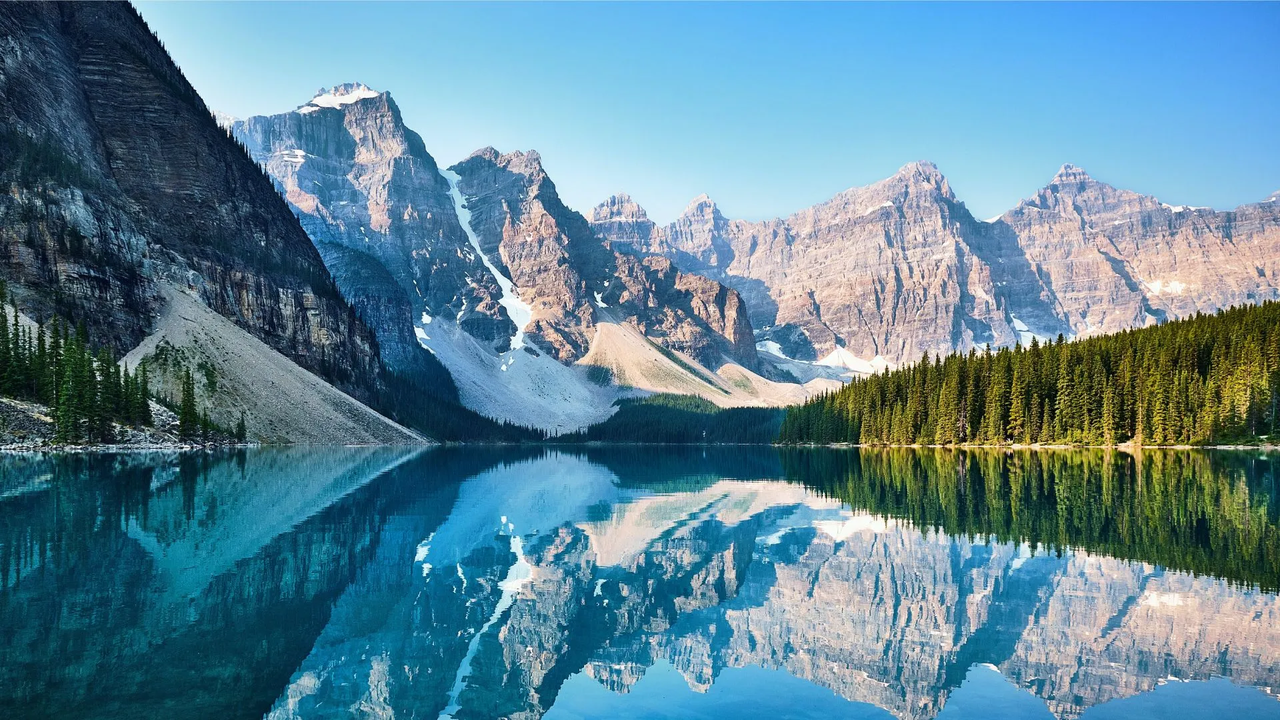
\includegraphics[width=7.5cm]{images/res/input_zip.png} }}%
	\qquad
	\subfloat[\centering Kết quả]{{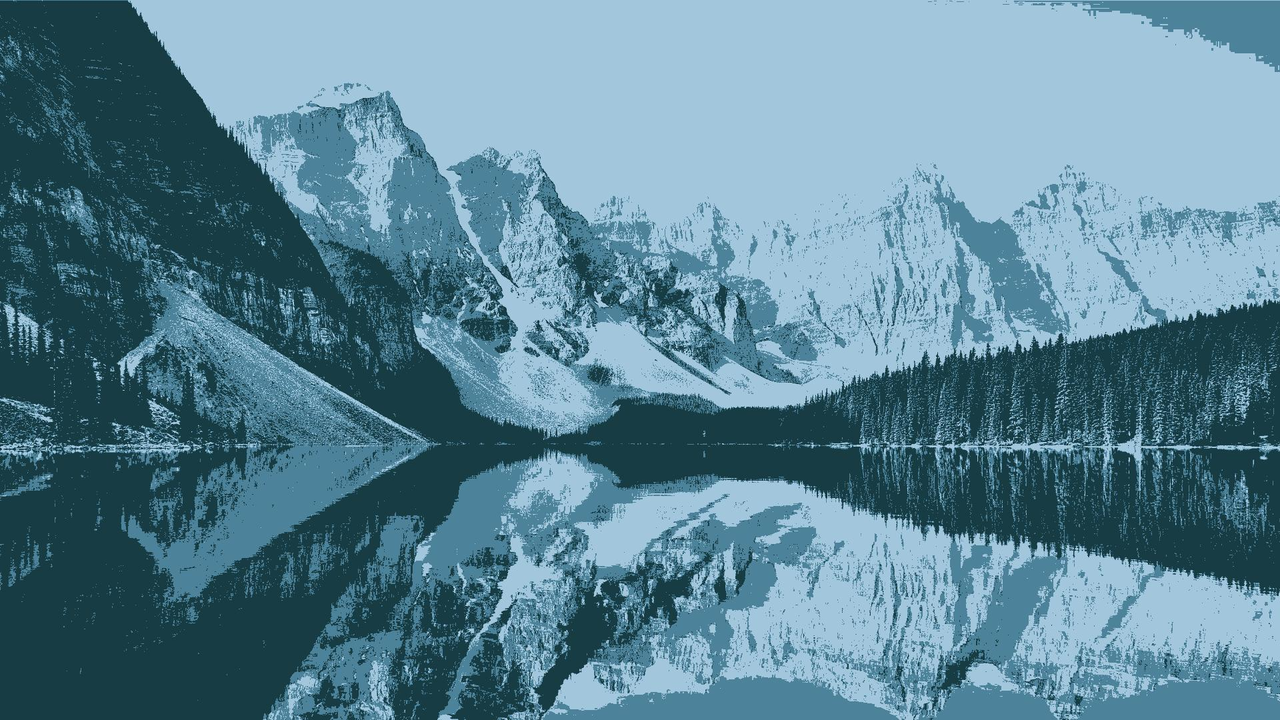
\includegraphics[width=7.5cm]{images/res/in_pixels_3_zip.png} }}%
	\caption{Kết quả với \texttt{init\_method = in\_pixels} và $K = 3$}%
\end{figure}

\subsubsection{Kết quả với giá trị $K = 5$}
\begin{figure}[H]
	\centering
	\subfloat[\centering Ảnh gốc]{{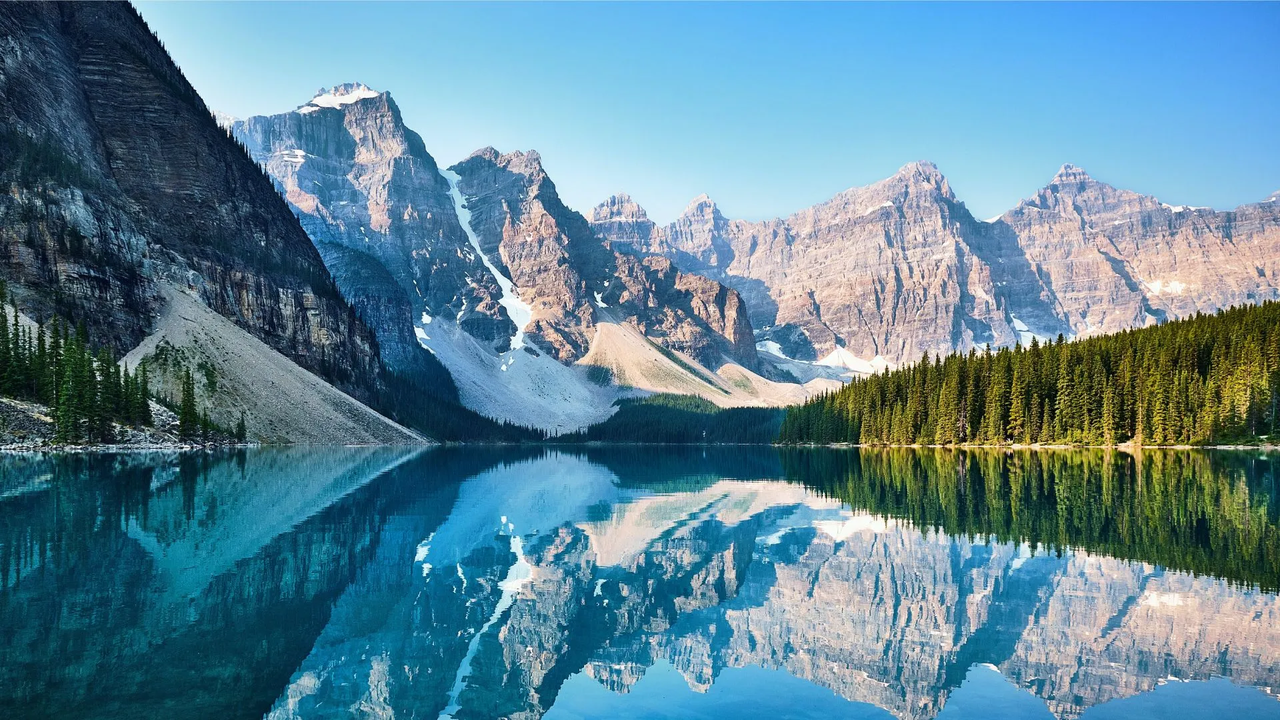
\includegraphics[width=7.5cm]{images/res/input_zip.png} }}%
	\qquad
	\subfloat[\centering Kết quả]{{
\includegraphics[width=7.5cm]{images/res/in_pixels_5_zip.png} }}%
	\caption{Kết quả với \texttt{init\_method = in\_pixels} và $K = 5$}%
\end{figure}

\subsubsection{Kết quả với giá trị $K = 7$}
\begin{figure}[H]
	\centering
	\subfloat[\centering Ảnh gốc]{{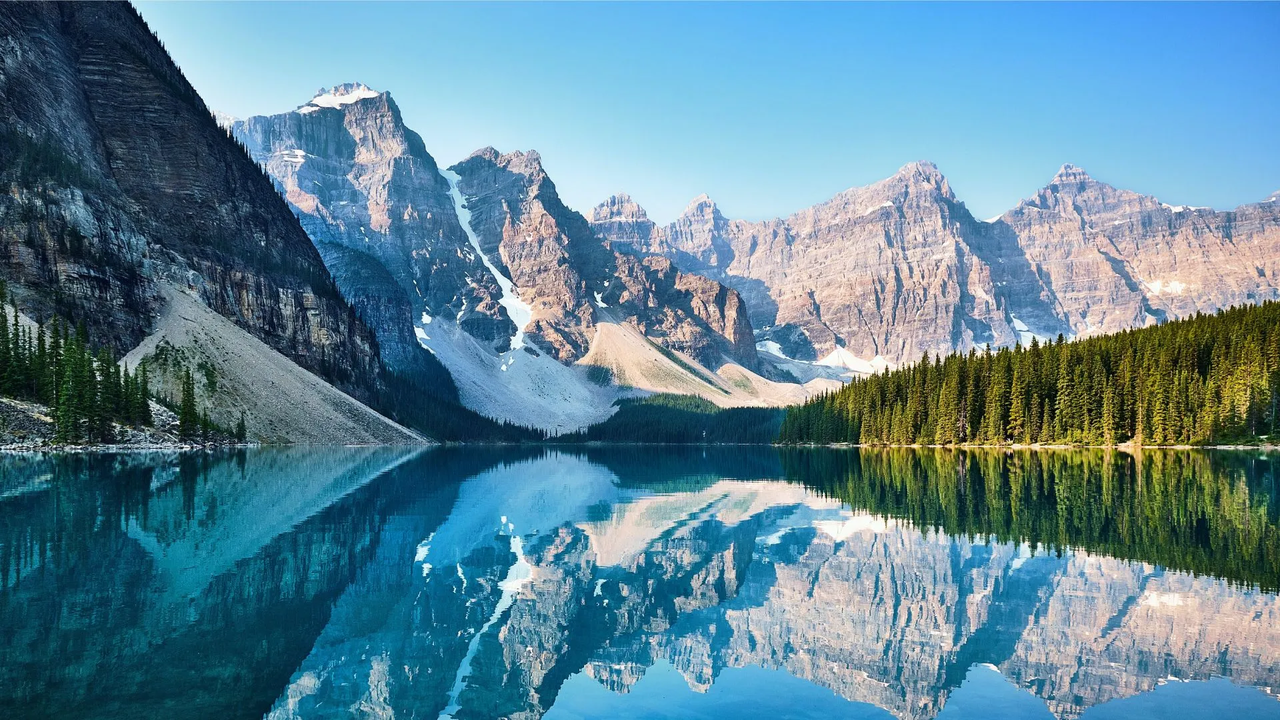
\includegraphics[width=7.5cm]{images/res/input_zip.png} }}%
	\qquad
	\subfloat[\centering Kết quả]{{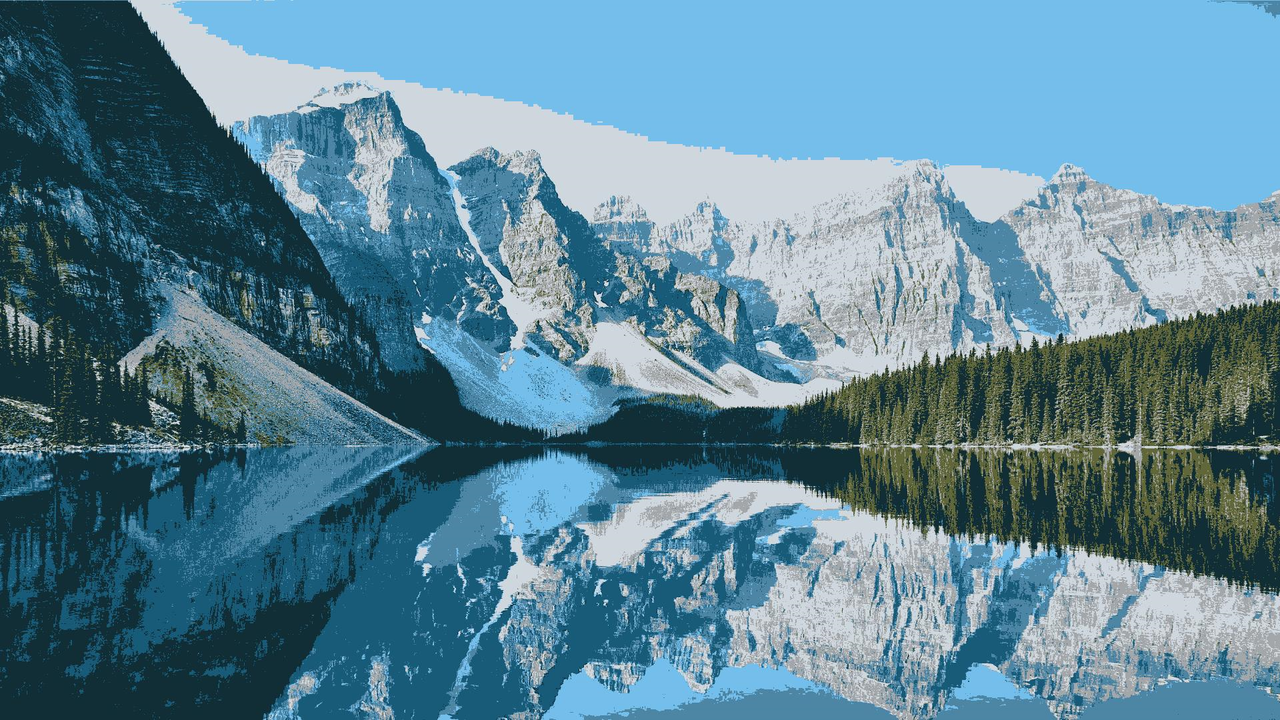
\includegraphics[width=7.5cm]{images/res/in_pixels_7_zip.png} }}%
	\caption{Kết quả với \texttt{init\_method = in\_pixels} và $K = 7$}%
\end{figure}

\subsubsection{Kết quả với giá trị $K = 9$}
\begin{figure}[H]
	\centering
	\subfloat[\centering Ảnh gốc]{{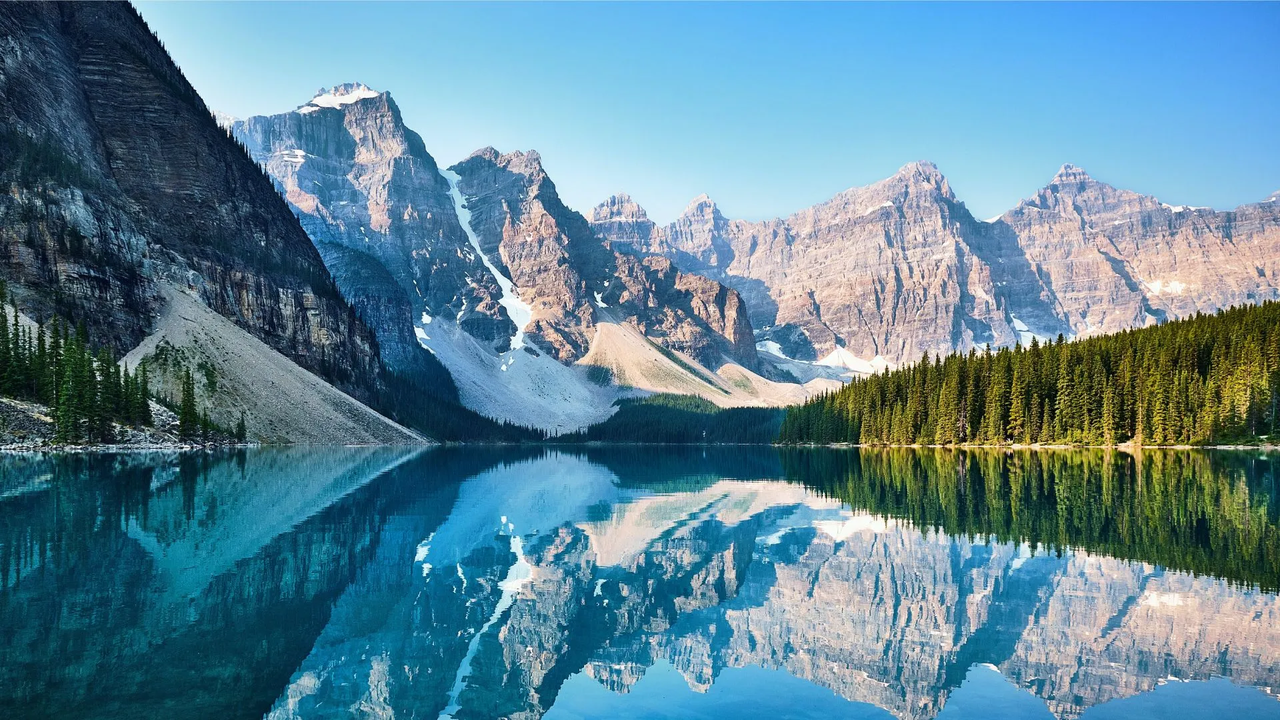
\includegraphics[width=7.5cm]{images/res/input_zip.png} }}%
	\qquad
	\subfloat[\centering Kết quả]{{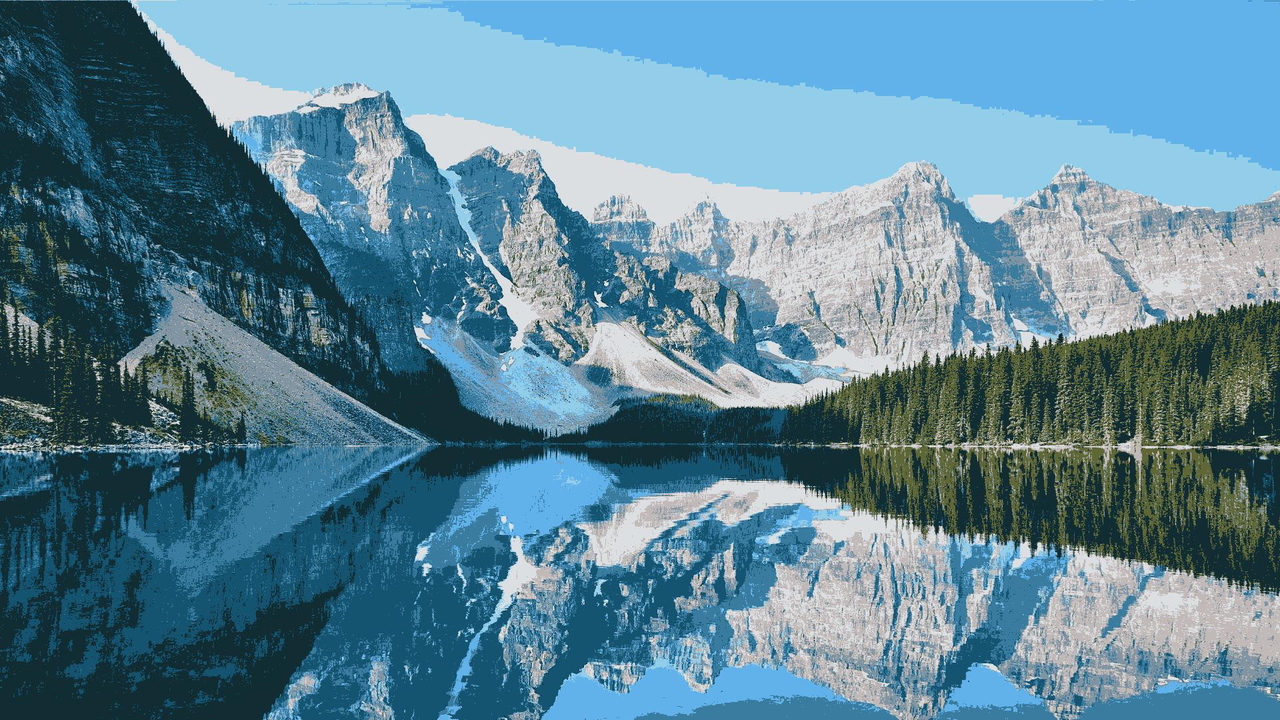
\includegraphics[width=7.5cm]{images/res/in_pixels_9_zip.png} }}%
	\caption{Kết quả với \texttt{init\_method = in\_pixels} và $K = 9$}%
\end{figure}

\subsection{Kết quả với init\_method = \texttt{random}}

\subsubsection{Kết quả với giá trị $K = 3$}
\begin{figure}[H]
	\centering
	\subfloat[\centering Ảnh gốc]{{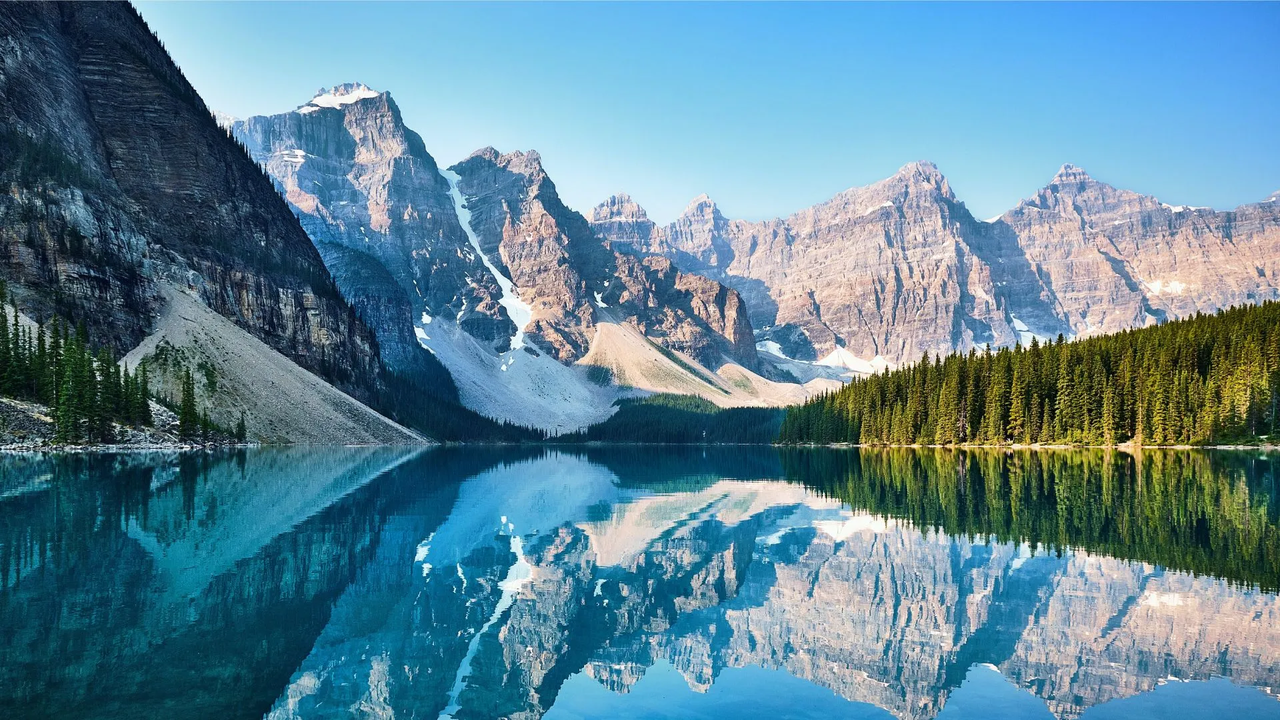
\includegraphics[width=7.5cm]{images/res/input_zip.png} }}%
	\qquad
	\subfloat[\centering Kết quả]{{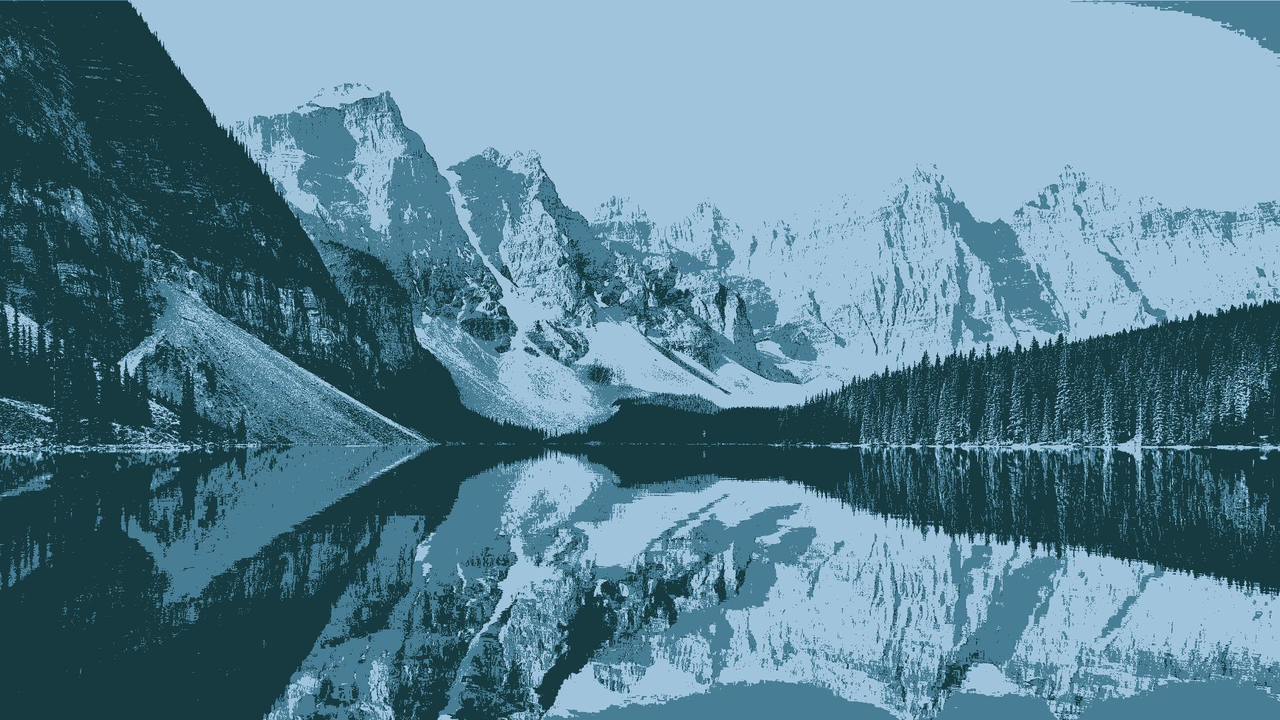
\includegraphics[width=7.5cm]{images/res/random_3_zip.png} }}%
	\caption{Kết quả với \texttt{init\_method = random} và $K = 3$}%
\end{figure}

\subsubsection{Kết quả với giá trị $K = 5$}
\begin{figure}[H]
	\centering
	\subfloat[\centering Ảnh gốc]{{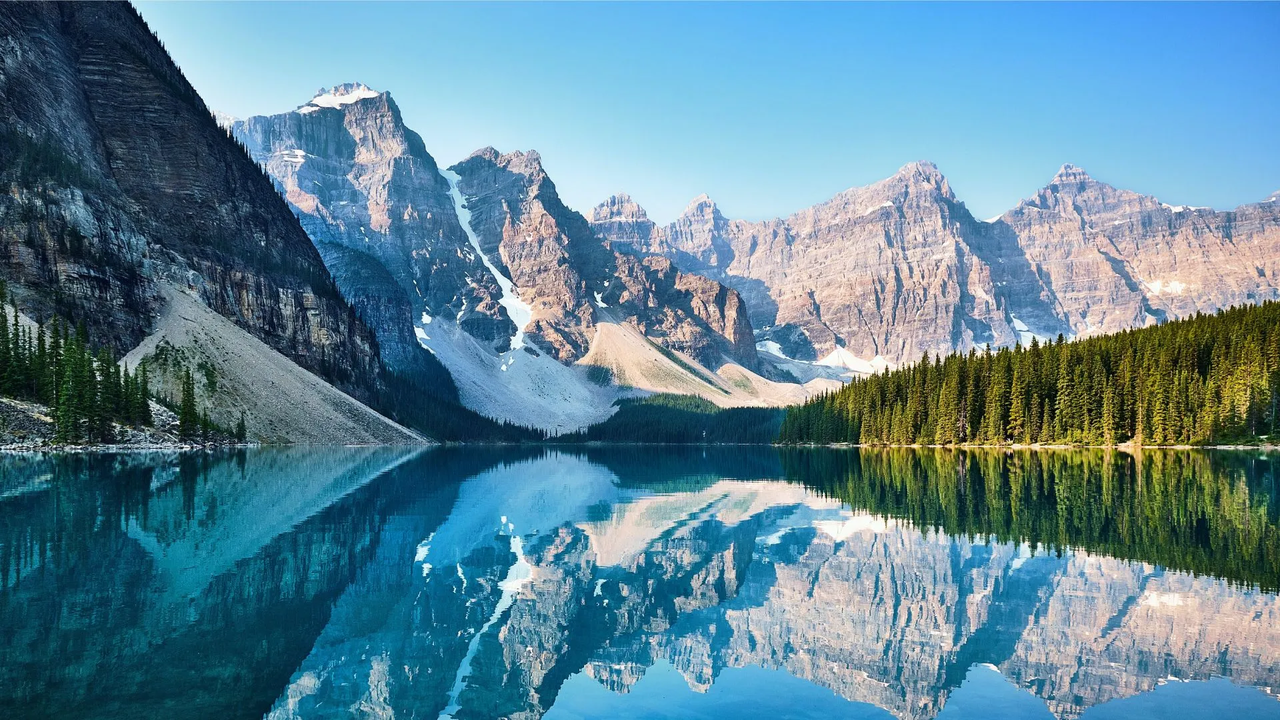
\includegraphics[width=7.5cm]{images/res/input_zip.png} }}%
	\qquad
	\subfloat[\centering Kết quả]{{
\includegraphics[width=7.5cm]{images/res/random_5_zip.png} }}%
	\caption{Kết quả với \texttt{init\_method = random} và $K = 5$}%
\end{figure}

\subsubsection{Kết quả với giá trị $K = 7$}
\begin{figure}[H]
	\centering
	\subfloat[\centering Ảnh gốc]{{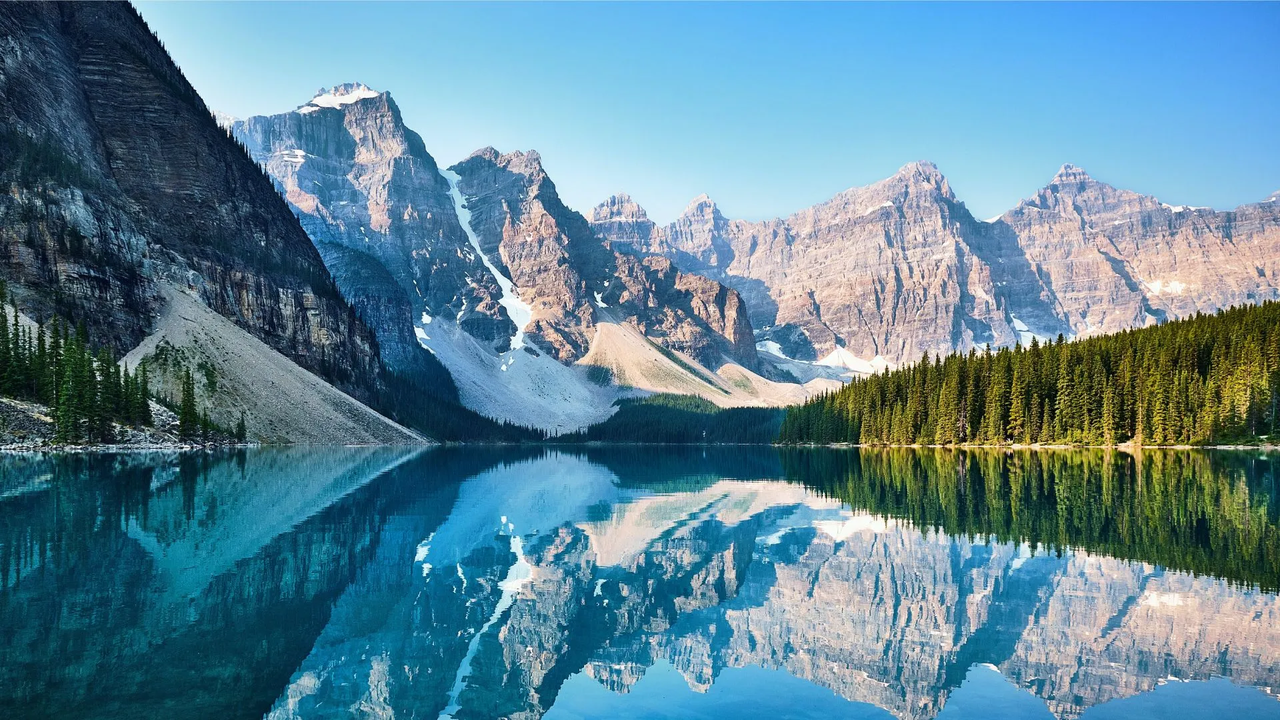
\includegraphics[width=7.5cm]{images/res/input_zip.png} }}%
	\qquad
	\subfloat[\centering Kết quả]{{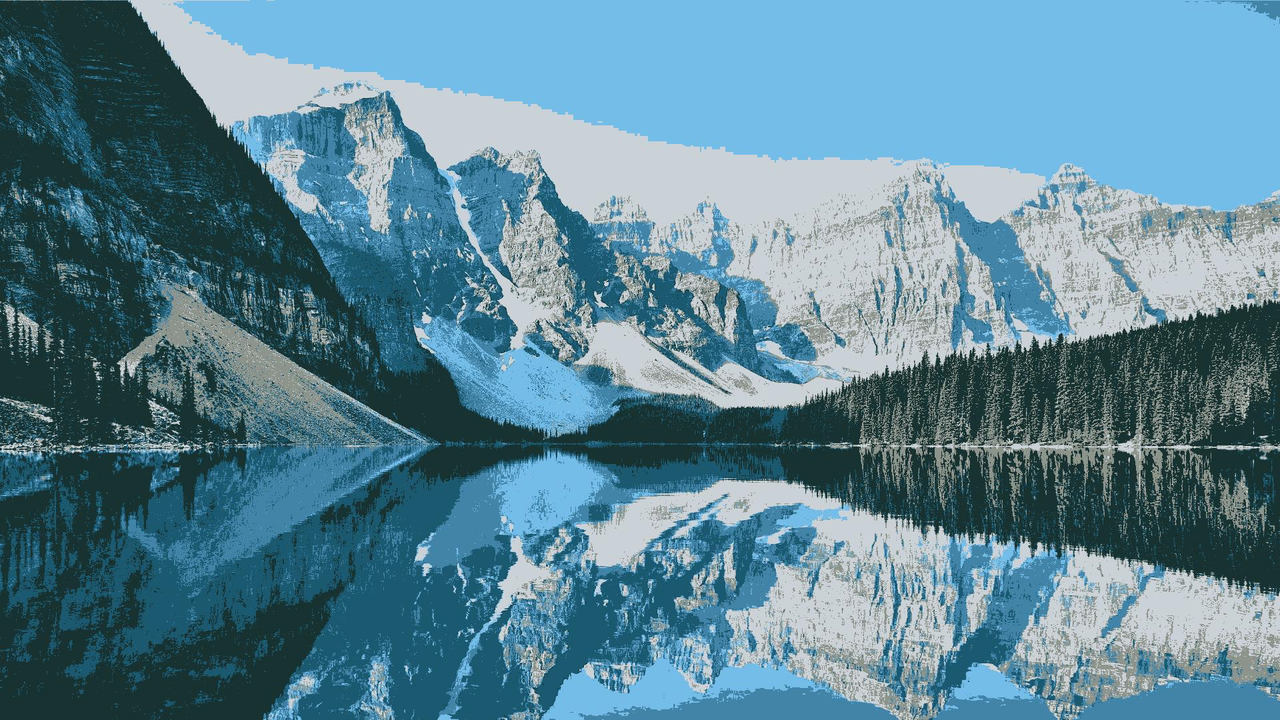
\includegraphics[width=7.5cm]{images/res/random_7_zip.png} }}%
	\caption{Kết quả với \texttt{init\_method = random} và $K = 7$}%
\end{figure}
\subsubsection{Kết quả với giá trị $K = 9$}
\begin{figure}[H]
	\centering
	\subfloat[\centering Ảnh gốc]{{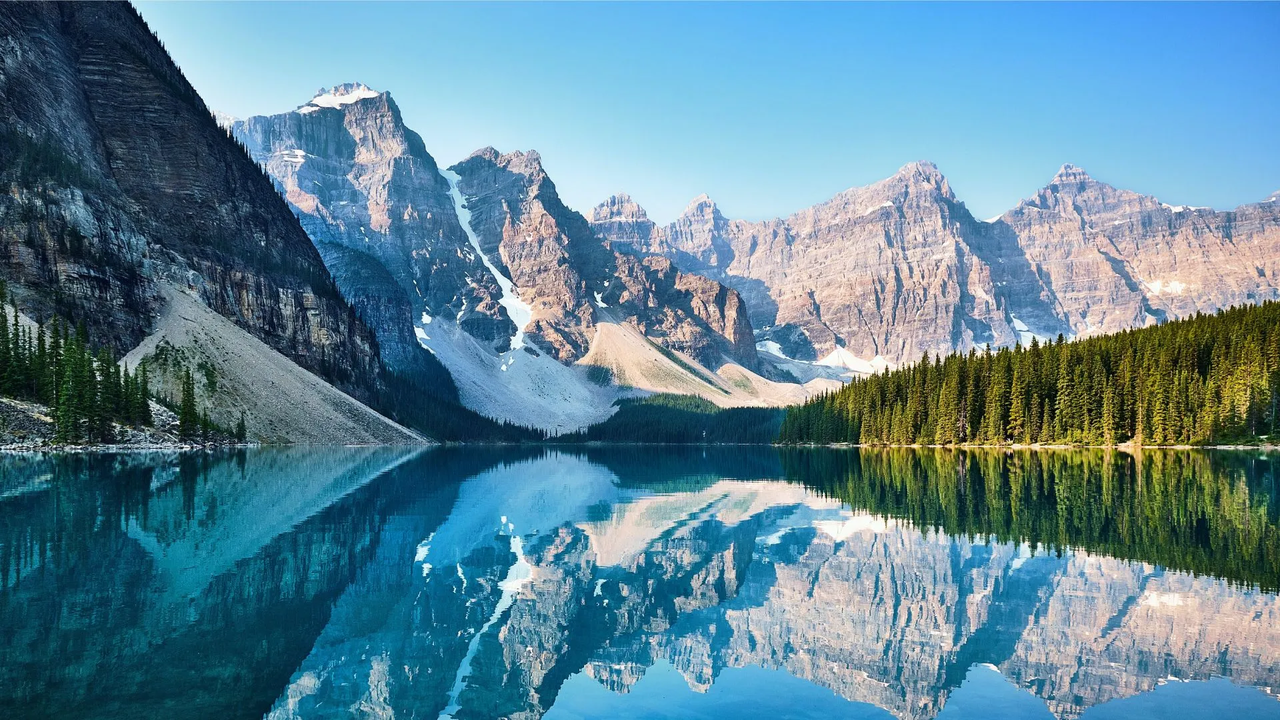
\includegraphics[width=7.5cm]{images/res/input_zip.png} }}%
	\qquad
	\subfloat[\centering Kết quả]{{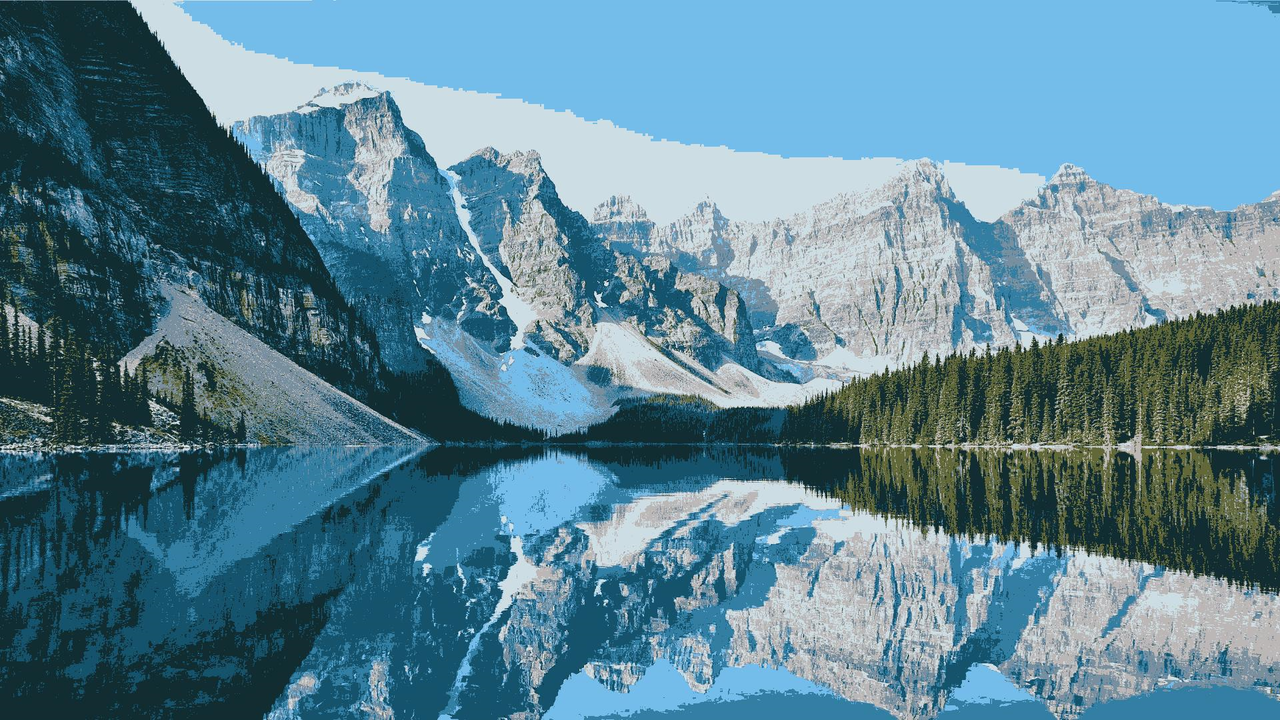
\includegraphics[width=7.5cm]{images/res/random_9_zip.png} }}%
	\caption{Kết quả với \texttt{init\_method = random} và $K = 9$}%
\end{figure}

\subsection{Thời gian thực hiện}

Để đánh giá thời gian thực hiện của thuật toán, ta sẽ đo thời gian thực hiện thuật toán với các phương pháp khởi tạo điểm centroid khác nhau và các giá trị $K$ khác nhau. Các kết quả được trình bày trong các hình bên dưới.
\begin{figure}[H]
	\centering
	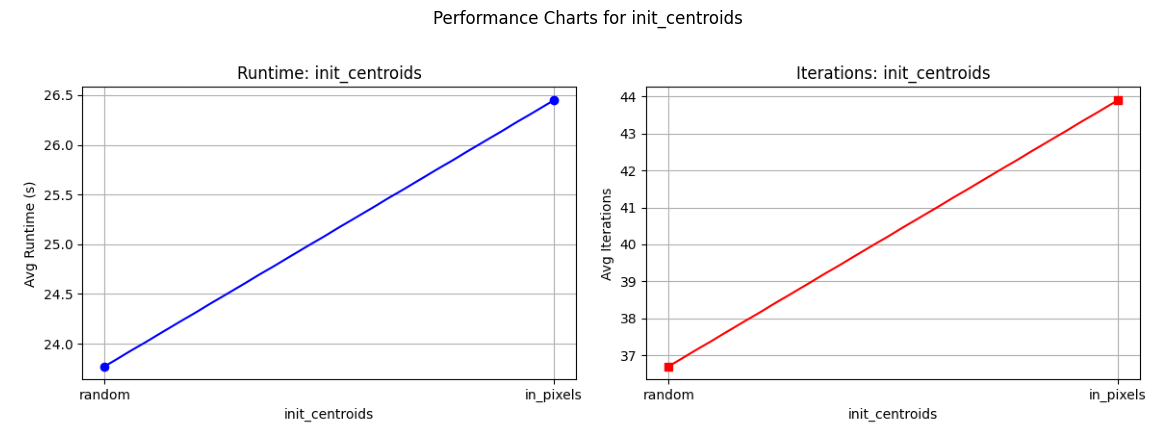
\includegraphics[width=\textwidth]{images/res/performance_init_centroids.png}
	\caption{Thời gian thực hiện thuật toán với các phương pháp khởi tạo điểm centroid khác nhau với $K = 5$ và $max\_iter = 100$}
\end{figure}

\begin{figure}[H]
	\centering
	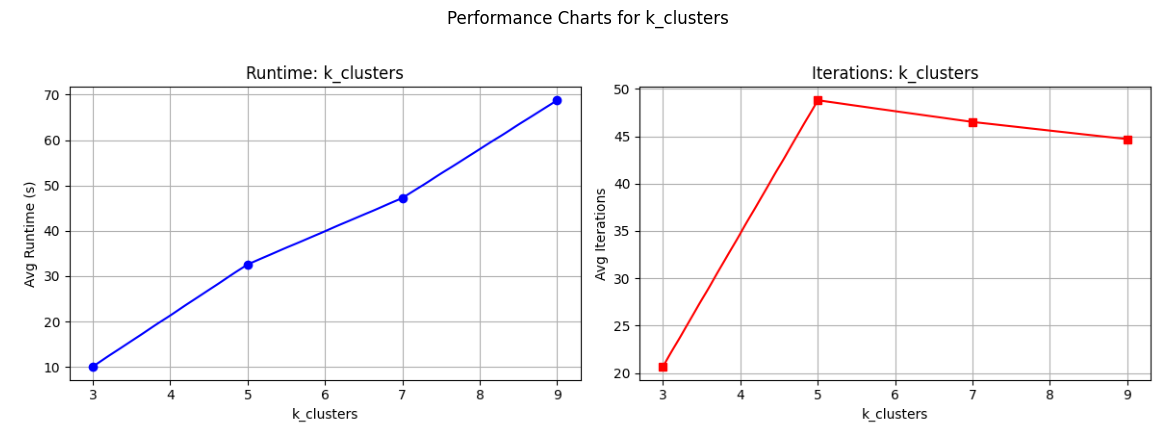
\includegraphics[width=\textwidth]{images/res/performance_k_clusters.png}
	\caption{Thời gian thực hiện thuật toán với các giá trị $K$ khác nhau với \texttt{init\_method = in\_pixels} và $max\_iter = 100$}
\end{figure}

\begin{figure}[H]
	\centering
	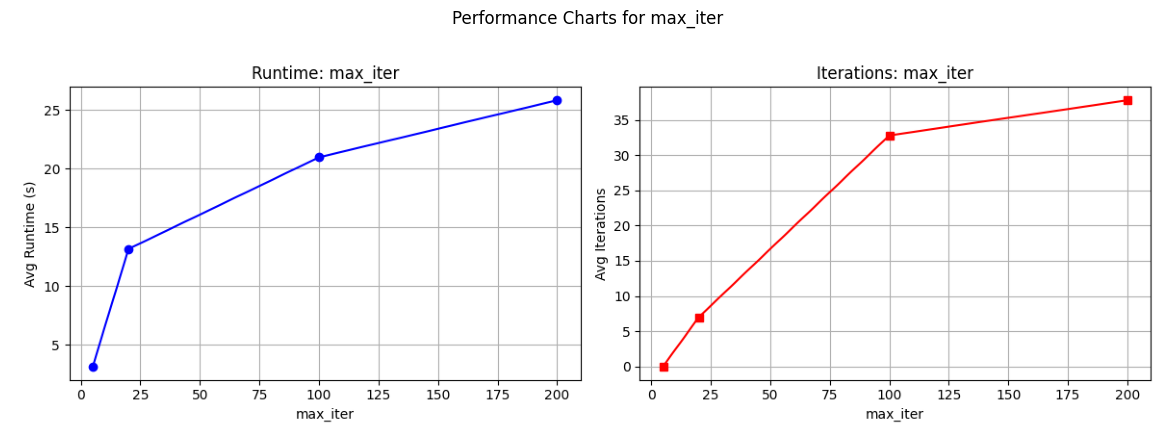
\includegraphics[width=\textwidth]{images/res/performance_max_iter.png}
	\caption{Thời gian thực hiện thuật toán với các giá trị $max\_iter$ khác nhau với \texttt{init\_method = in\_pixels} và $K = 5$}
\end{figure}
